\documentclass[tikz,border=10pt,10pt]{standalone}
\usepackage{tikz}
\usetikzlibrary{positioning, shapes.geometric, backgrounds, fit, arrows.meta}

\begin{document}

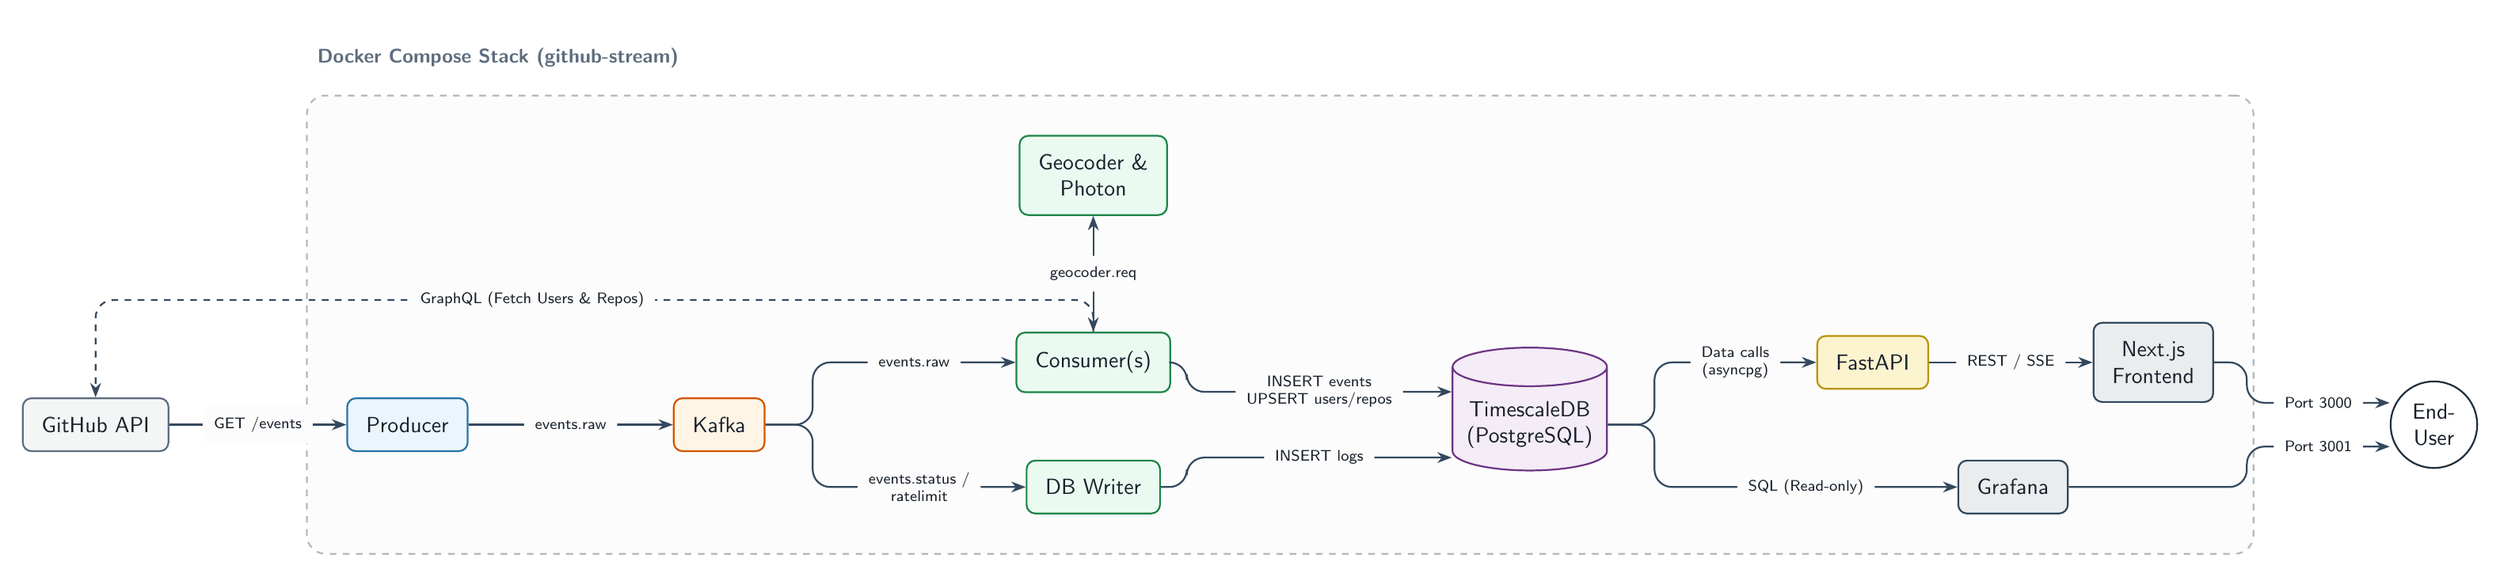
\begin{tikzpicture}[
    >=Stealth, % Stil der Pfeilspitzen
    % --- Farbdefinitionen aus dem wissenschaftlichen Theme ---
    extFill/.style={fill={rgb,255:red,244;green,246;blue,246}, draw={rgb,255:red,93;green,109;blue,126}},
    ingFill/.style={fill={rgb,255:red,235;green,245;blue,251}, draw={rgb,255:red,40;green,116;blue,166}},
    broFill/.style={fill={rgb,255:red,254;green,245;blue,231}, draw={rgb,255:red,211;green,84;blue,0}},
    proFill/.style={fill={rgb,255:red,234;green,250;blue,241}, draw={rgb,255:red,30;green,132;blue,73}},
    stoFill/.style={fill={rgb,255:red,244;green,236;blue,247}, draw={rgb,255:red,108;green,52;blue,131}},
    apiFill/.style={fill={rgb,255:red,252;green,243;blue,207}, draw={rgb,255:red,183;green,149;blue,11}},
    vizFill/.style={fill={rgb,255:red,234;green,236;blue,238}, draw={rgb,255:red,52;green,73;blue,94}},
    usrFill/.style={fill=white, draw={rgb,255:red,33;green,47;blue,61}},
    subFill/.style={fill={rgb,255:red,252;green,252;blue,252}},
    % --- Globale Node-Stile ---
    base/.style={thick, align=center, inner sep=2ex, rounded corners, text={rgb,255:red,23;green,32;blue,42}, font=\sffamily},
    database/.style={thick, align=center, inner sep=1.5ex, shape=cylinder, shape border rotate=90, aspect=0.25, minimum height=1.8cm, text={rgb,255:red,23;green,32;blue,42}, font=\sffamily},
    % --- Zuweisung der Stile ---
    external/.style={base, extFill},
    ingestion/.style={base, ingFill},
    broker/.style={base, broFill},
    processing/.style={base, proFill},
    storage/.style={database, stoFill},
    api/.style={base, apiFill},
    viz/.style={base, vizFill},
    userNode/.style={base, usrFill, shape=circle, inner sep=1ex},
    % --- Linienstile ---
    edge_style/.style={->, thick, draw={rgb,255:red,52;green,73;blue,94}},
    bidir_edge/.style={<->, thick, draw={rgb,255:red,52;green,73;blue,94}},
    % --- Beschriftungsstil (Hintergrund deckend, um Linien sauber zu durchbrechen) ---
    edge_label/.style={font=\scriptsize\sffamily, fill={rgb,255:red,252;green,252;blue,252}, inner sep=5pt, rounded corners=2pt, text={rgb,255:red,23;green,32;blue,42}, align=center}
]

    % ===========================
    % 1. PLATZIERUNG DER KNOTEN 
    % ===========================
    \node[external]   (GH)      at (0, 0)      {GitHub API};
    \node[ingestion]  (Prod)    at (5, 0)      {Producer};
    \node[broker]     (Kafka)   at (10, 0)     {Kafka};
    
    \node[processing] (Cons)    at (16, 1)     {Consumer(s)};
    \node[processing] (Geo)     at (16, 4)     {Geocoder \&\\Photon};
    \node[processing] (DBW)     at (16, -1)    {DB Writer};
    
    \node[storage]    (DB)      at (23, 0)     {TimescaleDB\\(PostgreSQL)};
    
    \node[api]        (API)     at (28.5, 1)     {FastAPI};
    \node[viz]        (Front)   at (33, 1)     {Next.js\\Frontend};
    \node[viz]        (Grafana) at (30.75, -1)    {Grafana};
    
    \node[userNode]   (User)    at (37.5, 0)     {End-\\User};

    % ===========================
    % 2. VERBINDUNGEN (Pfeile an das neue kompakte Raster angepasst)
    % ===========================
    
    % GitHub -> Producer
    \draw[edge_style] (GH.east) -- node[edge_label] {GET /events} (Prod.west);

    % GraphQL Call: Consumer -> GitHub API (angepasste Breite auf X=16 und Höhe Y=8.5)
    \draw[edge_style, dashed, rounded corners=8pt] (Cons.north) -- (16, 2) -- (14, 2) -- node[edge_label] {GraphQL (Fetch Users \& Repos)} (0, 2) -- (GH.north);

    % Producer -> Kafka
    \draw[edge_style] (Prod.east) -- node[edge_label] {events.raw} (Kafka.west);

    % Kafka -> Consumer & DB Writer (Knick in der Mitte bei X=13.5)
    \draw[edge_style, rounded corners=8pt] (Kafka.east) -- (11.5, 0) -- (11.5, 1) -- node[edge_label] {events.raw} (Cons.west);
    \draw[edge_style, rounded corners=8pt] (Kafka.east) -- (11.5, 0) -- (11.5, -1) -- node[edge_label] {events.status /\\ratelimit} (DBW.west);

    % Consumer <-> Geocoder
    \draw[bidir_edge] (Cons.north) -- node[edge_label] {geocoder.req} (Geo.south);

    % Consumer & DB Writer -> Datenbank (Knick in der Mitte bei X=18.5)
    \draw[edge_style, rounded corners=8pt] (Cons.east) -- (17.5, 1) -- (17.5, 15pt) -- node[edge_label] {INSERT events\\UPSERT users/repos} ([yshift=15pt]DB.west);
    \draw[edge_style, rounded corners=8pt] (DBW.east) -- (17.5, -1) -- (17.5, -15pt) -- node[edge_label] {INSERT logs} ([yshift=-15pt]DB.west);

    % Datenbank -> API & Grafana (Knick in der Mitte bei X=23.5)
    \draw[edge_style, rounded corners=8pt] ([yshift=0pt]DB.east) -- (25, 0pt) -- (25, 1) -- node[edge_label] {Data calls\\(asyncpg)} (API.west);
    \draw[edge_style, rounded corners=8pt] ([yshift=-0pt]DB.east) -- (25, -0pt) -- (25, -1) -- node[edge_label] {SQL (Read-only)} (Grafana.west);

    % API -> Frontend
    \draw[edge_style] (API.east) -- node[edge_label] {REST / SSE} (Front.west);

    % Frontend & Grafana -> Endbenutzer (Knick in der Mitte bei X=34)
    \draw[edge_style, rounded corners=8pt] (Front.east) -- (34.5, 1) -- (34.5, 10pt) -- node[edge_label, fill=white] {Port 3000} ([yshift=10pt]User.west);
    \draw[edge_style, rounded corners=8pt] (Grafana.east) -- (34.5, -1) -- (34.5, -10pt) -- node[edge_label, fill=white] {Port 3001} ([yshift=-10pt]User.west);

    % ===========================
    % 3. SUBGRAPH (DOCKER STACK)
    % ===========================
    \begin{scope}[on background layer]
        % Box, die alle internen Komponenten umschließt
        \node[subFill, draw={rgb,255:red,178;green,186;blue,187}, thick, dashed, rounded corners=3mm, inner sep=18pt, 
              fit=(Prod) (Kafka) (Cons) (Geo) (DBW) (DB) (API) (Grafana) (Front)] (box) {};
              
        % Beschriftung der Box (oben links)
        \node[anchor=south west, font=\sffamily\bfseries\small, text={rgb,255:red,93;green,109;blue,126}, inner xsep=5pt, inner ysep=12pt] 
        at (box.north west) {Docker Compose Stack (github-stream)};
    \end{scope}

\end{tikzpicture}

\end{document}